%\documentclass[notes,10pt,aspectratio=169]{beamer}

%\documentclass[notes, 10pt,aspectratio=169]{beamer}
\documentclass[10pt,aspectratio=169]{beamer}


% Add this line to your preamble
%\setbeameroption{show notes on second screen=right}

%\usetheme{Singapore} %Boadilla, Madrid, default, etc. 
\usetheme[progressbar=frametitle]{metropolis}
\usecolortheme{rose} %beaver, dolphin, crane, 


%\setbeamersize{text margin left=4mm, text margin right=4mm}


\usecolortheme{default}

\usepackage[utf8]{inputenc}
\usepackage[T1]{fontenc}
\usepackage{lmodern}
\usepackage{xcolor}
\usepackage{tikz}
\usepackage{booktabs} % Required for \toprule, \midrule, \bottomrule
\usetikzlibrary{shapes.geometric, arrows, positioning}

\tikzstyle{block} = [rectangle, draw, text width=4cm, align=center, rounded corners, minimum height=1cm]
\tikzstyle{decision} = [rectangle, draw, text width=5cm, align=center, fill=blue!10, rounded corners, minimum height=1cm]
\tikzstyle{terminal} = [rectangle, draw, text width=4.5cm, align=center, fill=yellow!30, rounded corners, minimum height=1cm]
\tikzstyle{end} = [rectangle, draw, text width=5cm, align=center, fill=green!30, rounded corners, minimum height=1cm]
\tikzstyle{arrow} = [->, thick]



\usepackage{adjustbox}
%2. change the bullets 
\setbeamertemplate{itemize item}[triangle] %circle, square,... 


% 1. Define custom colors and set colors 
%\definecolor{myblue}{HTML}{003366}
\definecolor{accent}{RGB}{78,205,196}

%\setbeamercolor{title}{fg=white,bg=myblue}
\setbeamercolor{frametitle}{fg=black,bg=white}
%\setbeamercolor{normal text}{fg=mygray}
\setbeamercolor{block title}{fg=black,bg=blue}
%\setbeamercolor{block body}{fg=black,bg=white}

\setbeamercolor{item}{fg= orange!80} % Change bullet color
\setbeamercolor{button}{bg=orange, fg=white}





% 3. BibLaTeX settings
\usepackage[
  backend=biber,
  style=apa,
  citestyle=authoryear
]{biblatex}
\addbibresource{references.bib}

\title{Meetin with SPoints to discuss with Steve}
%\subtitle{A Mini Literature Overview}

\author{%
 Lucas Condeza
\inst{1} \and
   %\and
%  Coauthor Three\inst{3}
}
\institute{
  \inst{1} Yale University \\
}

\date{\today}

\begin{document}

%\begin{frame}
%  \titlepage
%\end{frame}






\begin{frame}{Previous meeting}

 \begin{itemize}
        \item Discussed the possible research questions including: what is the impact of information provision on equilibrium outcomes. 
        \item  
        \item  
\end{itemize}
\end{frame}


\begin{frame}{This meeting: topics}

 \begin{itemize}
        \item There is selection among firms. 
        \item Discuss model to study information issues. 
\end{itemize}
\end{frame}


\begin{frame}{Selection}
Selection? some firms better at predicting? 
 \begin{figure}
     \centering
     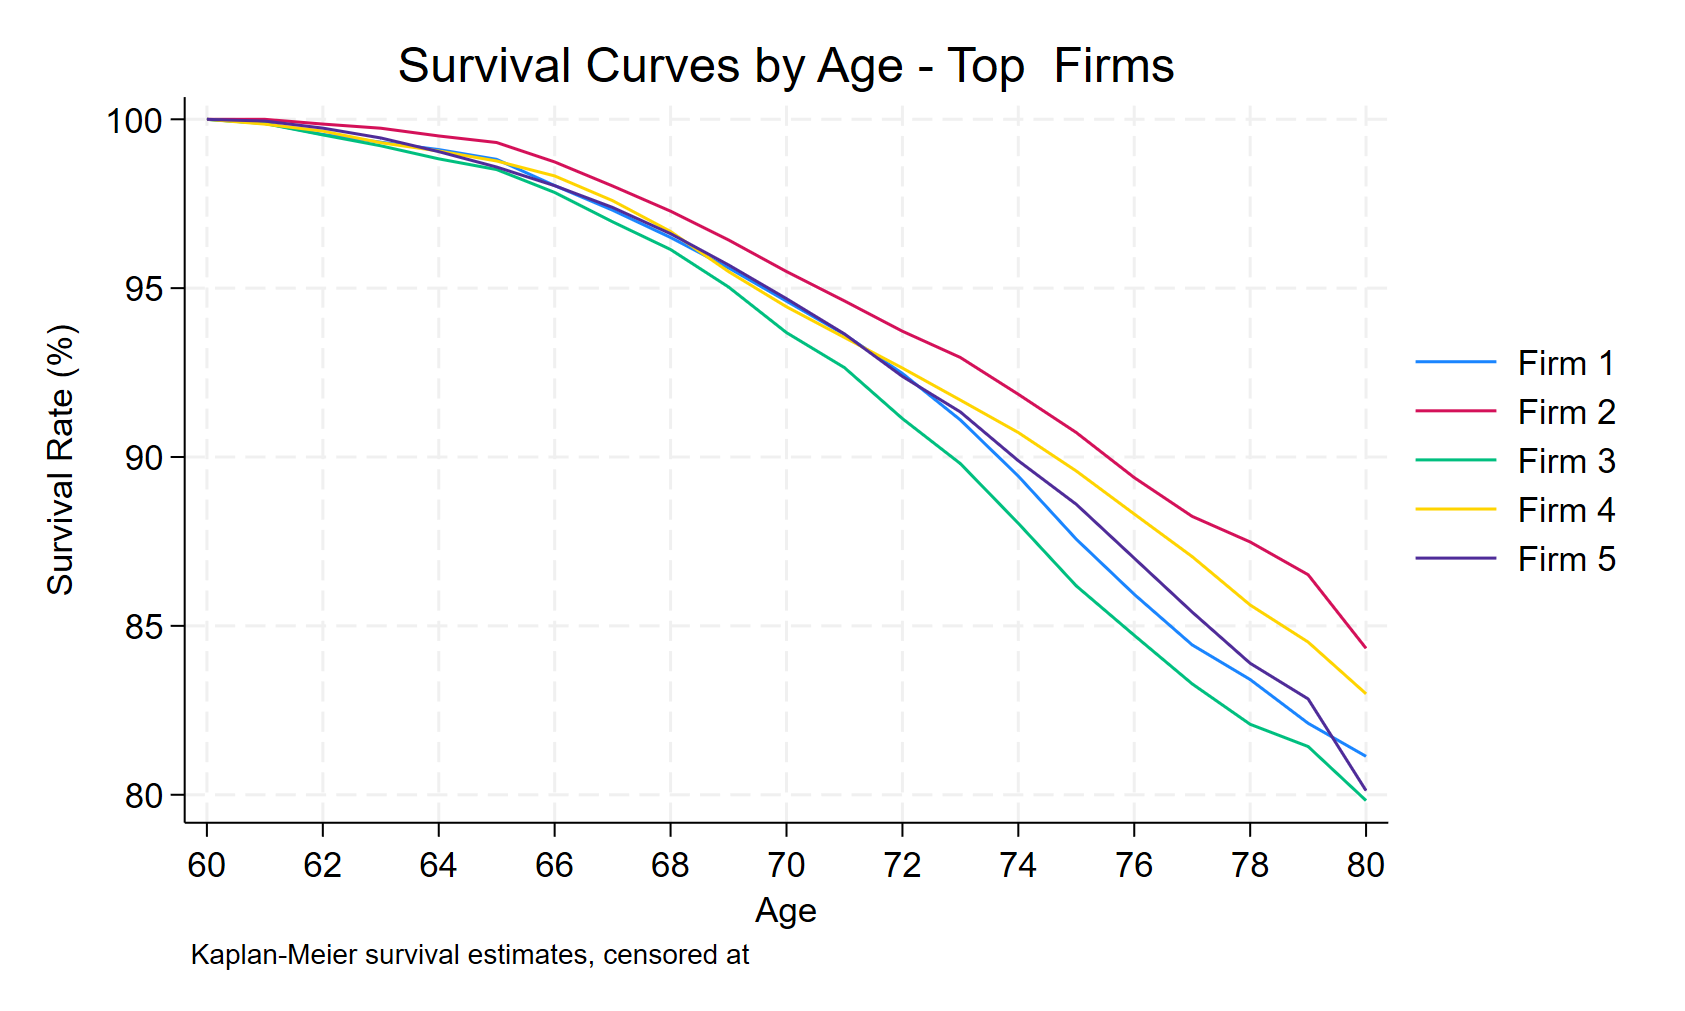
\includegraphics[width=0.6\linewidth]{figures//IE4/IE4_survival_curves_by_age_top_firms.png}
     %\caption{Enter Caption}
     \label{fig:placeholder}
 \end{figure}
Claim: one needs to observe the information observed by the firm to determine if there is selection -> 

In an exchange 
\end{frame}


\begin{frame}{Model(1)}
\begin{itemize}
    \item Nested logit model of a selection market (costs depend on unobserved health). 
    \item Ruled out selection across insurers by assuming mean utilities: $\delta_j - \alpha p_j + f(h)$
    \item Results: 
    \begin{enumerate}
        \item Selection into the market generates a higher average than marginal cost. 
        \item If the cost functions are not firm specific the average costs across firms are the same 
        \item Marginal costs are different even when 
        If the cost functions are not firm specific the average costs across firms are the same 
    \end{enumerate}
\end{itemize}
\end{frame}


\begin{frame}{Model(2)}
 \begin{figure}
     \centering
     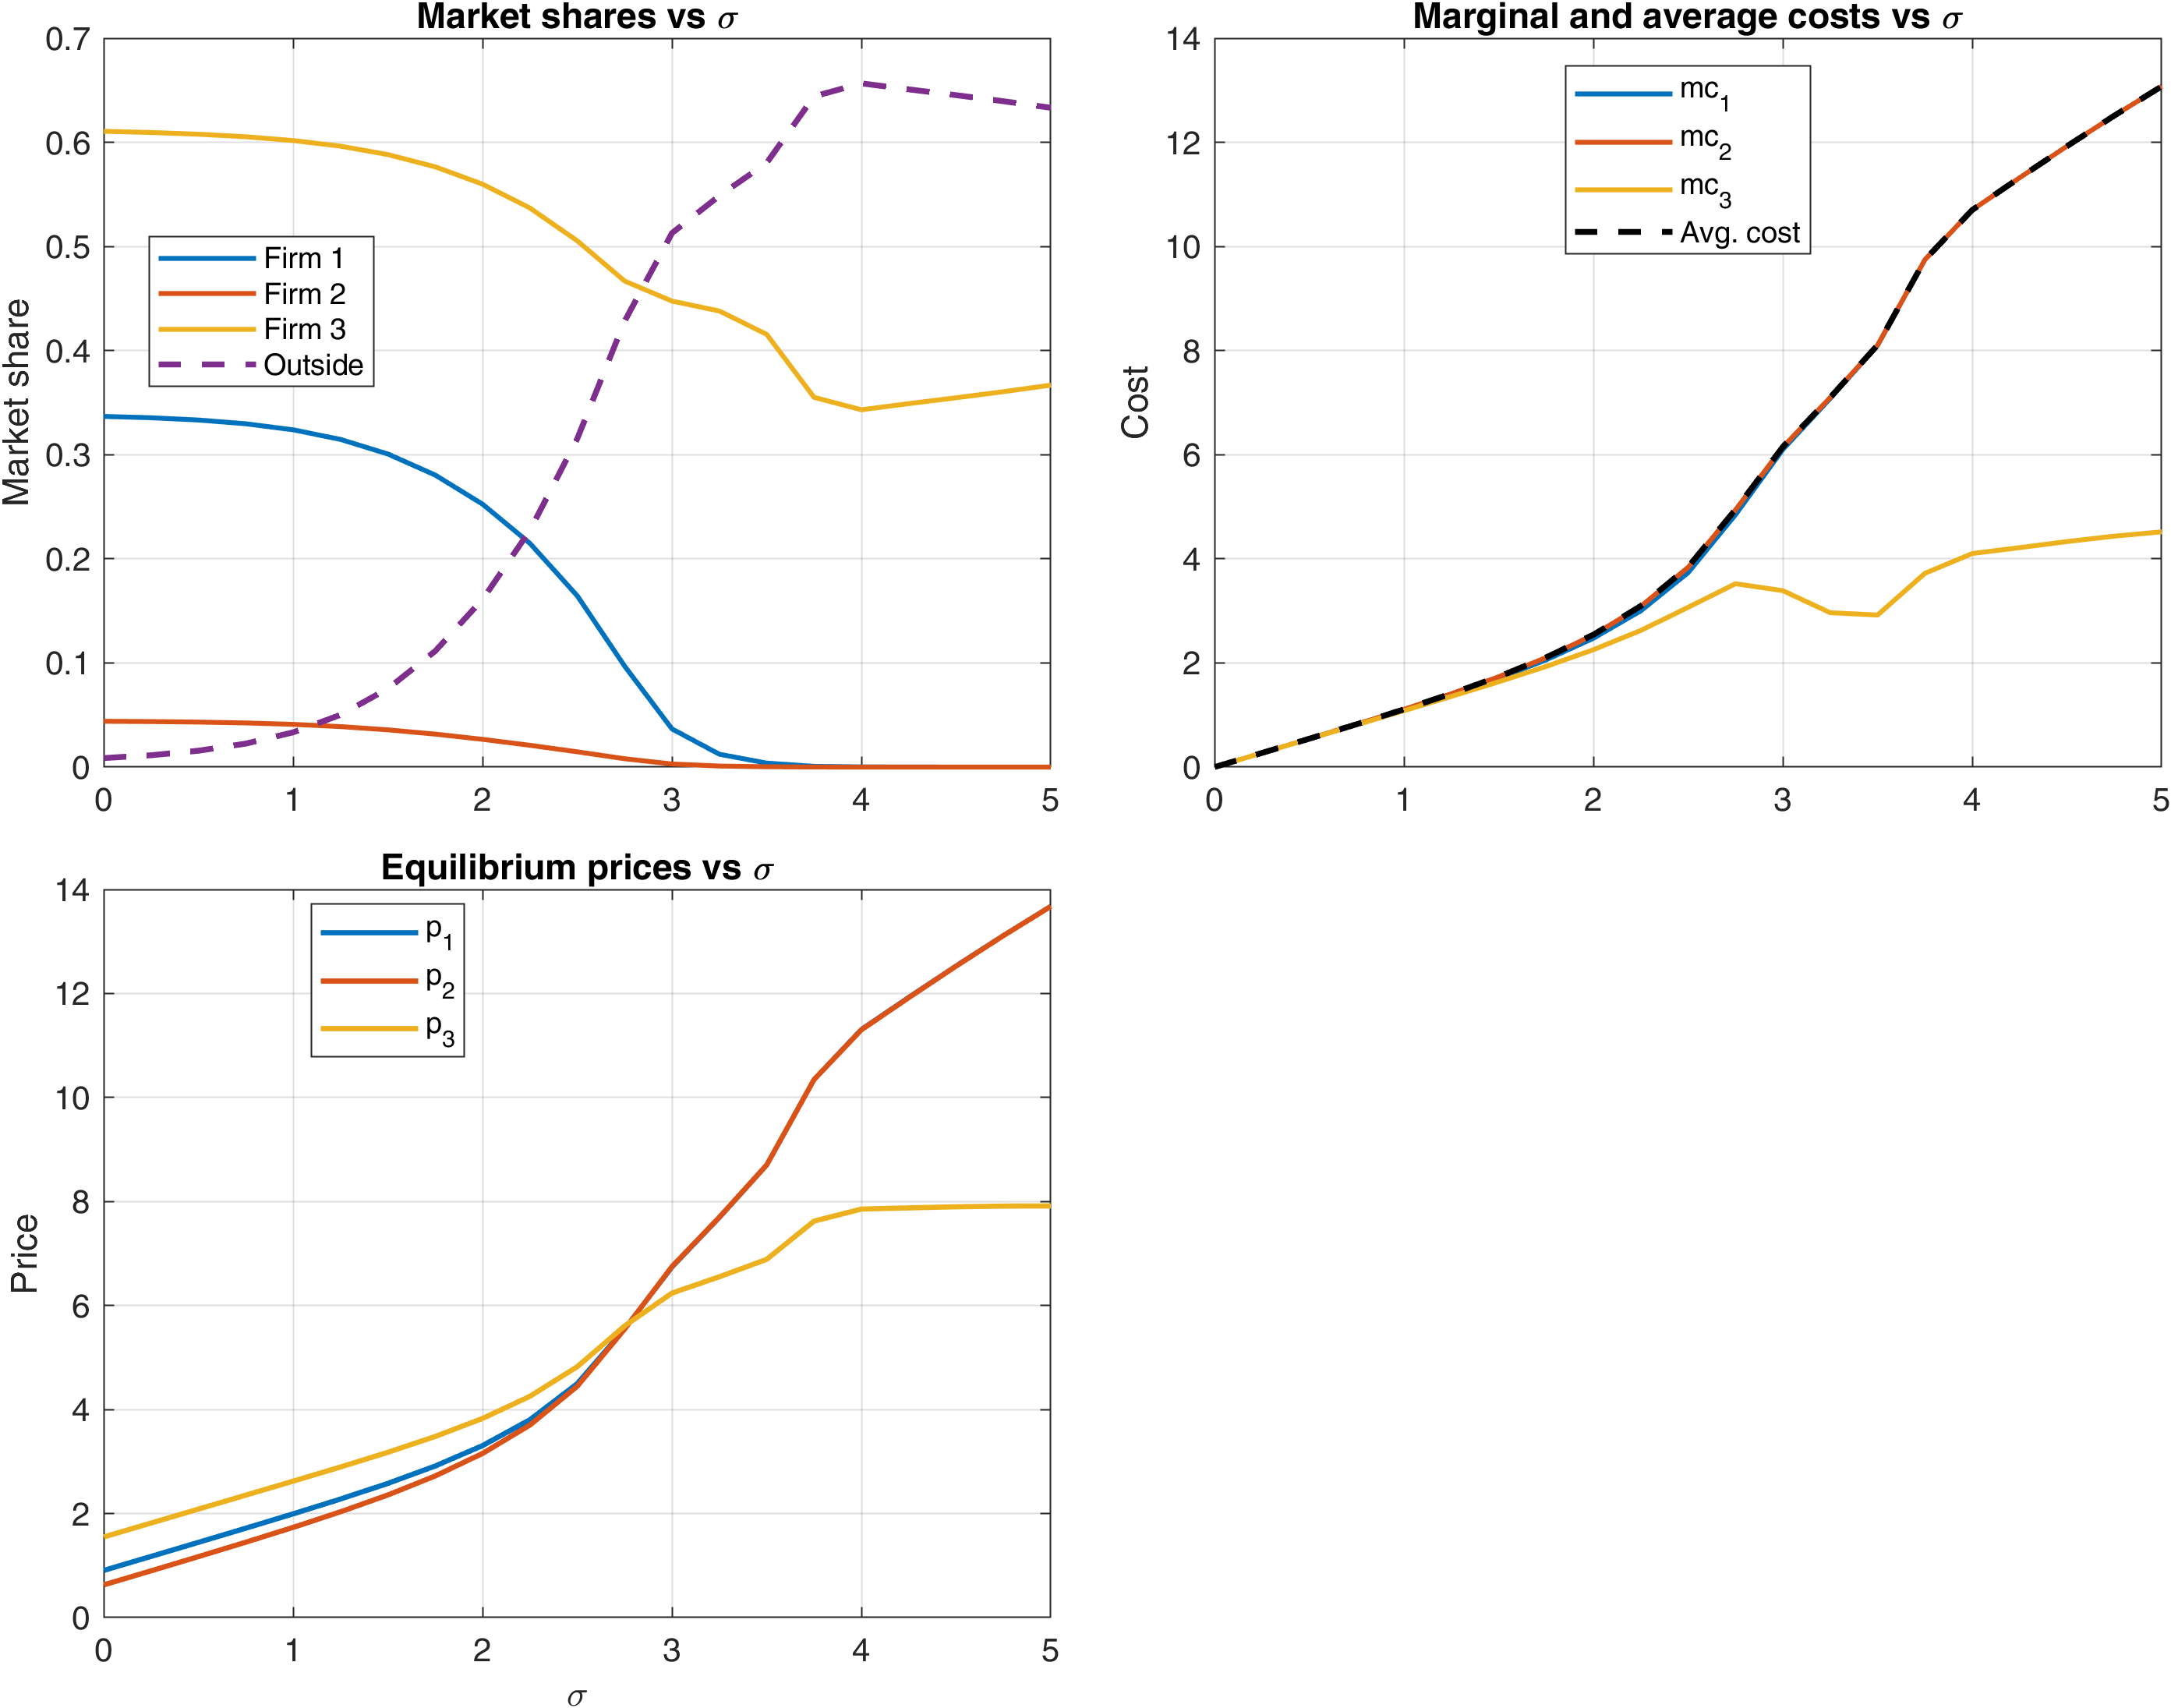
\includegraphics[width=0.6\linewidth]{figures/simulations/sigma_panels.png}
     %\caption{Enter Caption}
     \label{fig:placeholder}
 \end{figure}
\end{frame}

\begin{frame}{Caveats}
\begin{itemize}
    \item The model is appropriate to study  a particular pre-defined segment of the population.
    \item Is not the correct model to do comparative statics on $\sigma$. When changing $\sigma$ we are changing the cost distribution over the whole population, hence it is not correct to interpret it as just an informational intervention. 
\end{itemize}


\end{frame}



 
\end{document}